\begin{figure}[htbp]
    \centering
    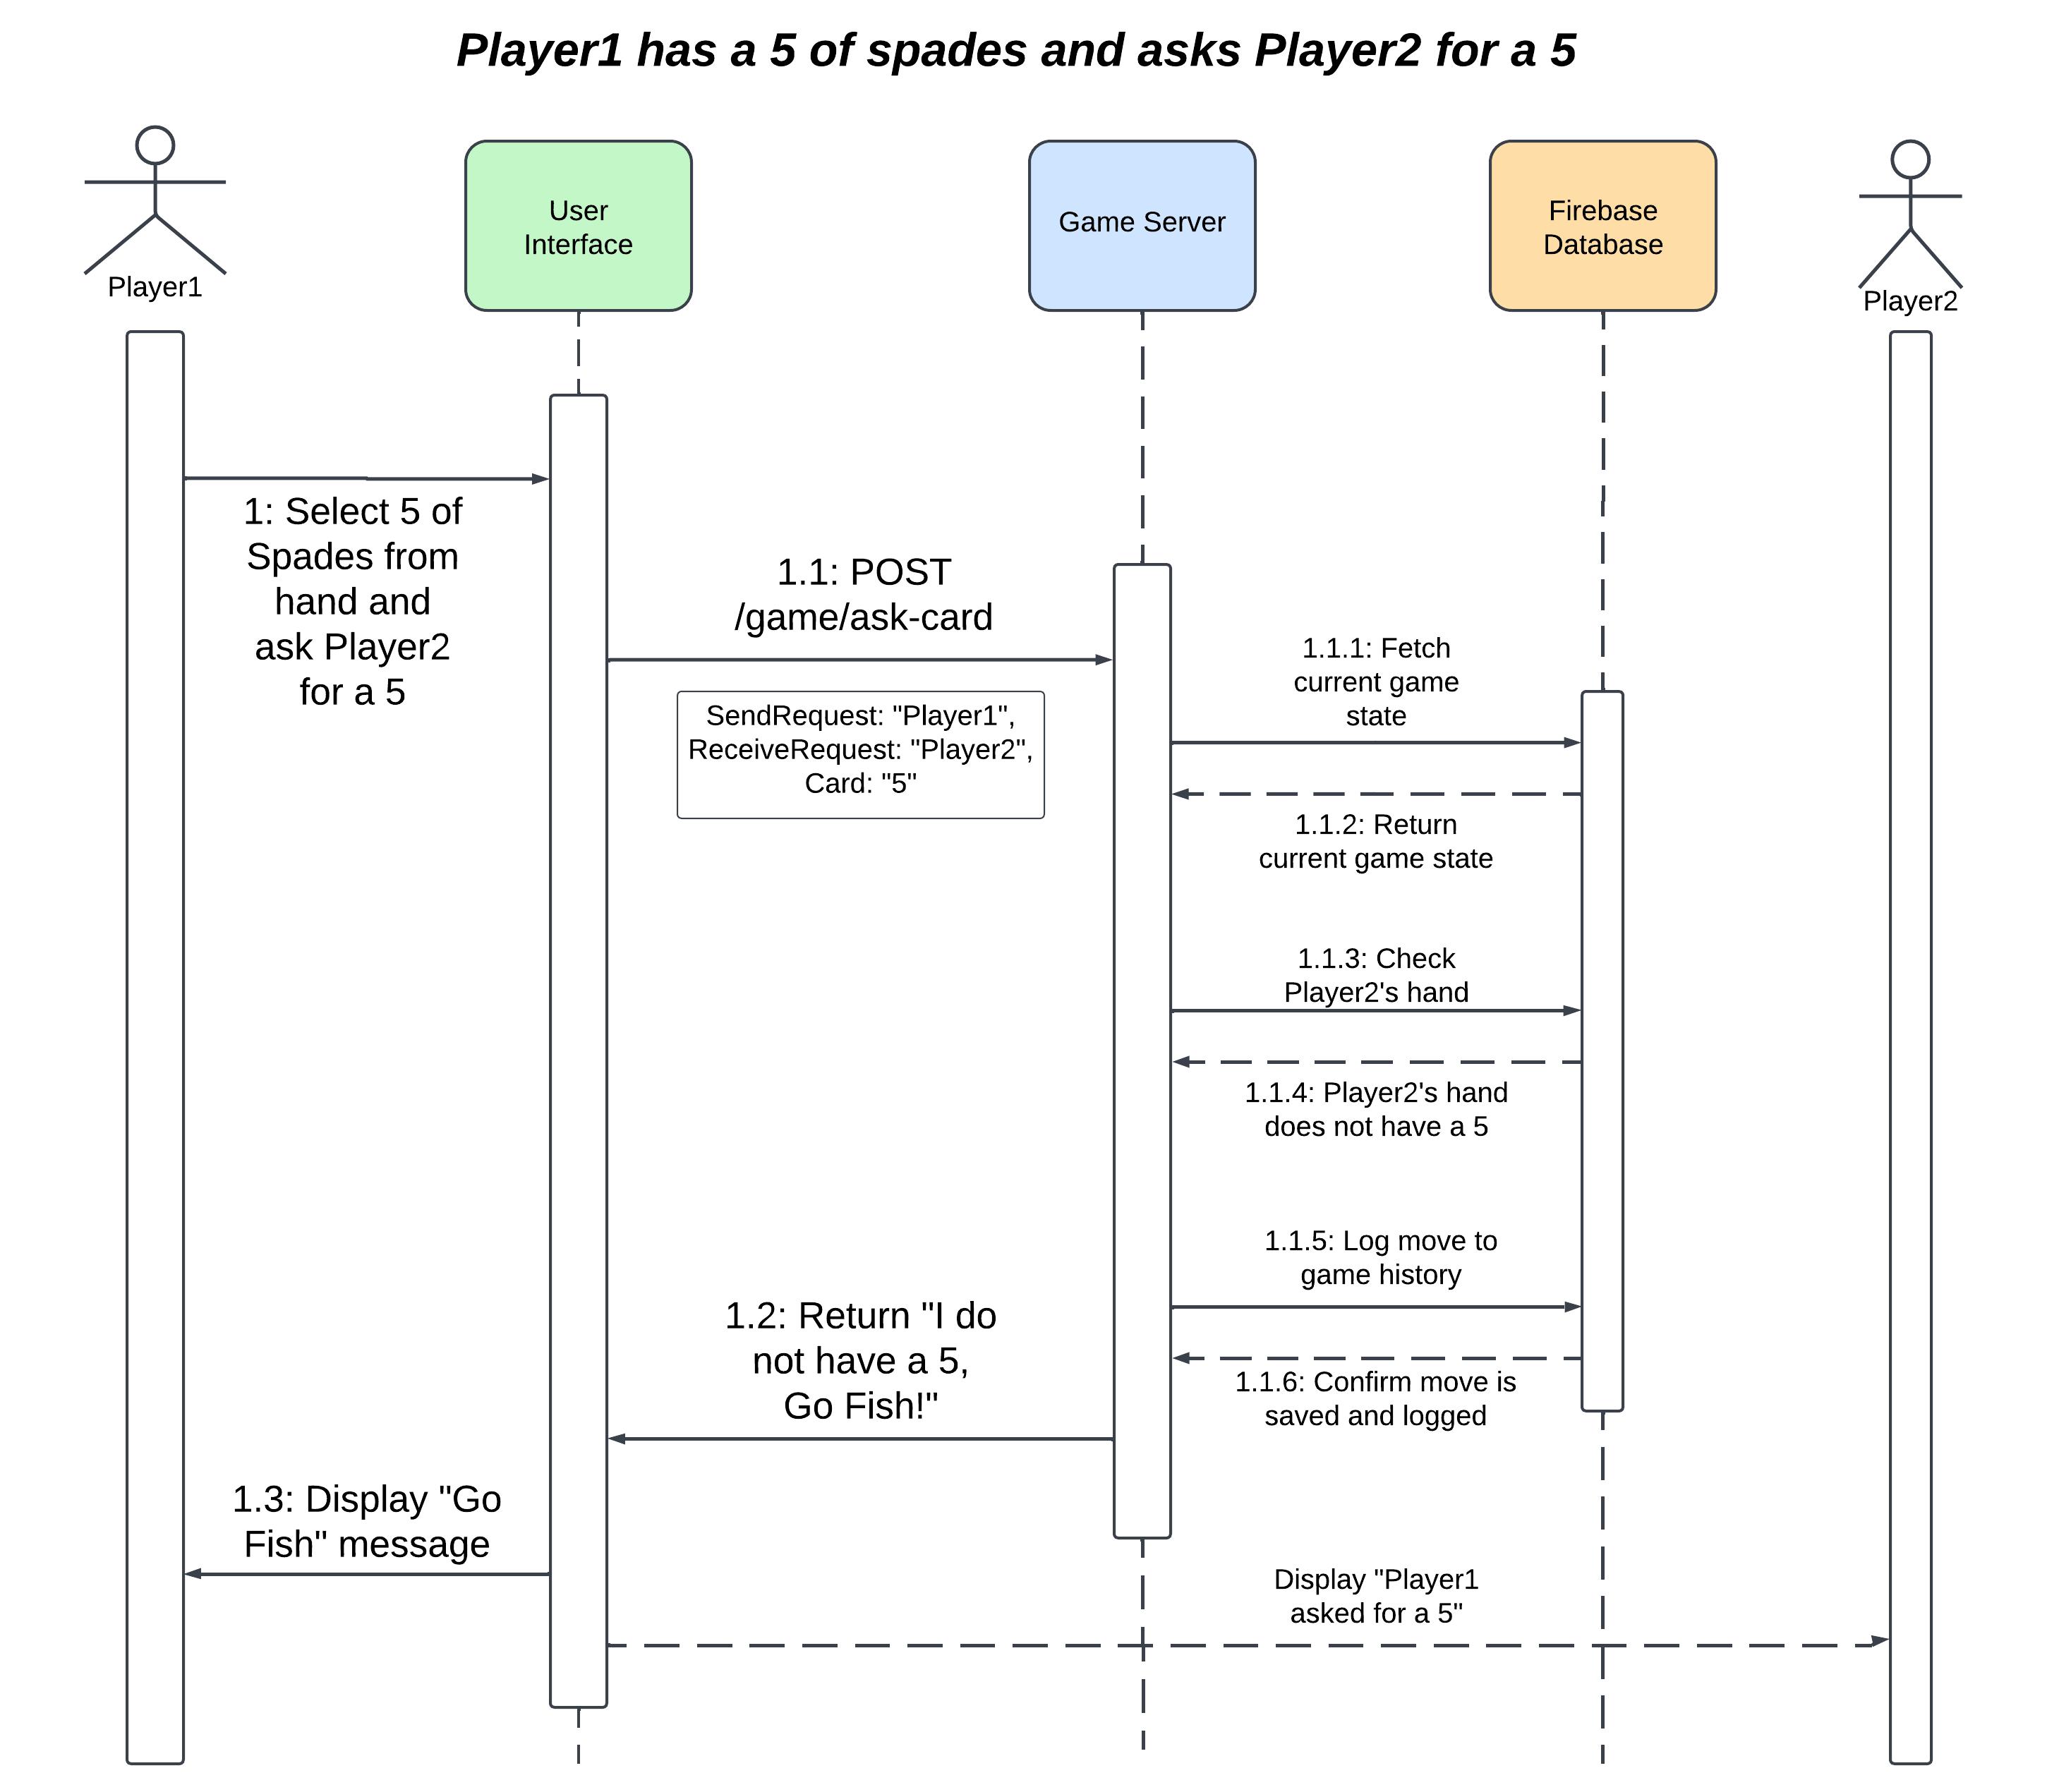
\includegraphics[width=1\linewidth]{CS482 Sequence Diagram Sprint 2.png}
    \caption{UML sequence diagram of Player1 asking Player2 for a card they do not have, resulting in Player1 being told to "Go Fish"}
    \label{fig:umlsequence}
\end{figure}

\noindent This UML sequence diagram illustrates the process of a player asking for a specific card during gameplay. In this scenario, Player1 selects a 5 of Spades from their hand and asks Player2 if they have any cards of the same rank. Player2, however, does not possess a 5, leading to the "Go Fish!" outcome for Player1.

\noindent The sequence begins with Player1 selecting the card and initiating a request through the game's user interface. This request is sent to the game server, which forwards it to the database to fetch Player2's current hand. The database responds with the data, enabling the server to check if Player2 has a 5. Upon finding that Player2 does not have the requested card, the server logs the move, saves the interaction in the game history, and returns a response to the user interface indicating that Player1 must "Go Fish!" The user interface then displays this message, completing the sequence.

\begin{figure}[htbp]
    \centering
    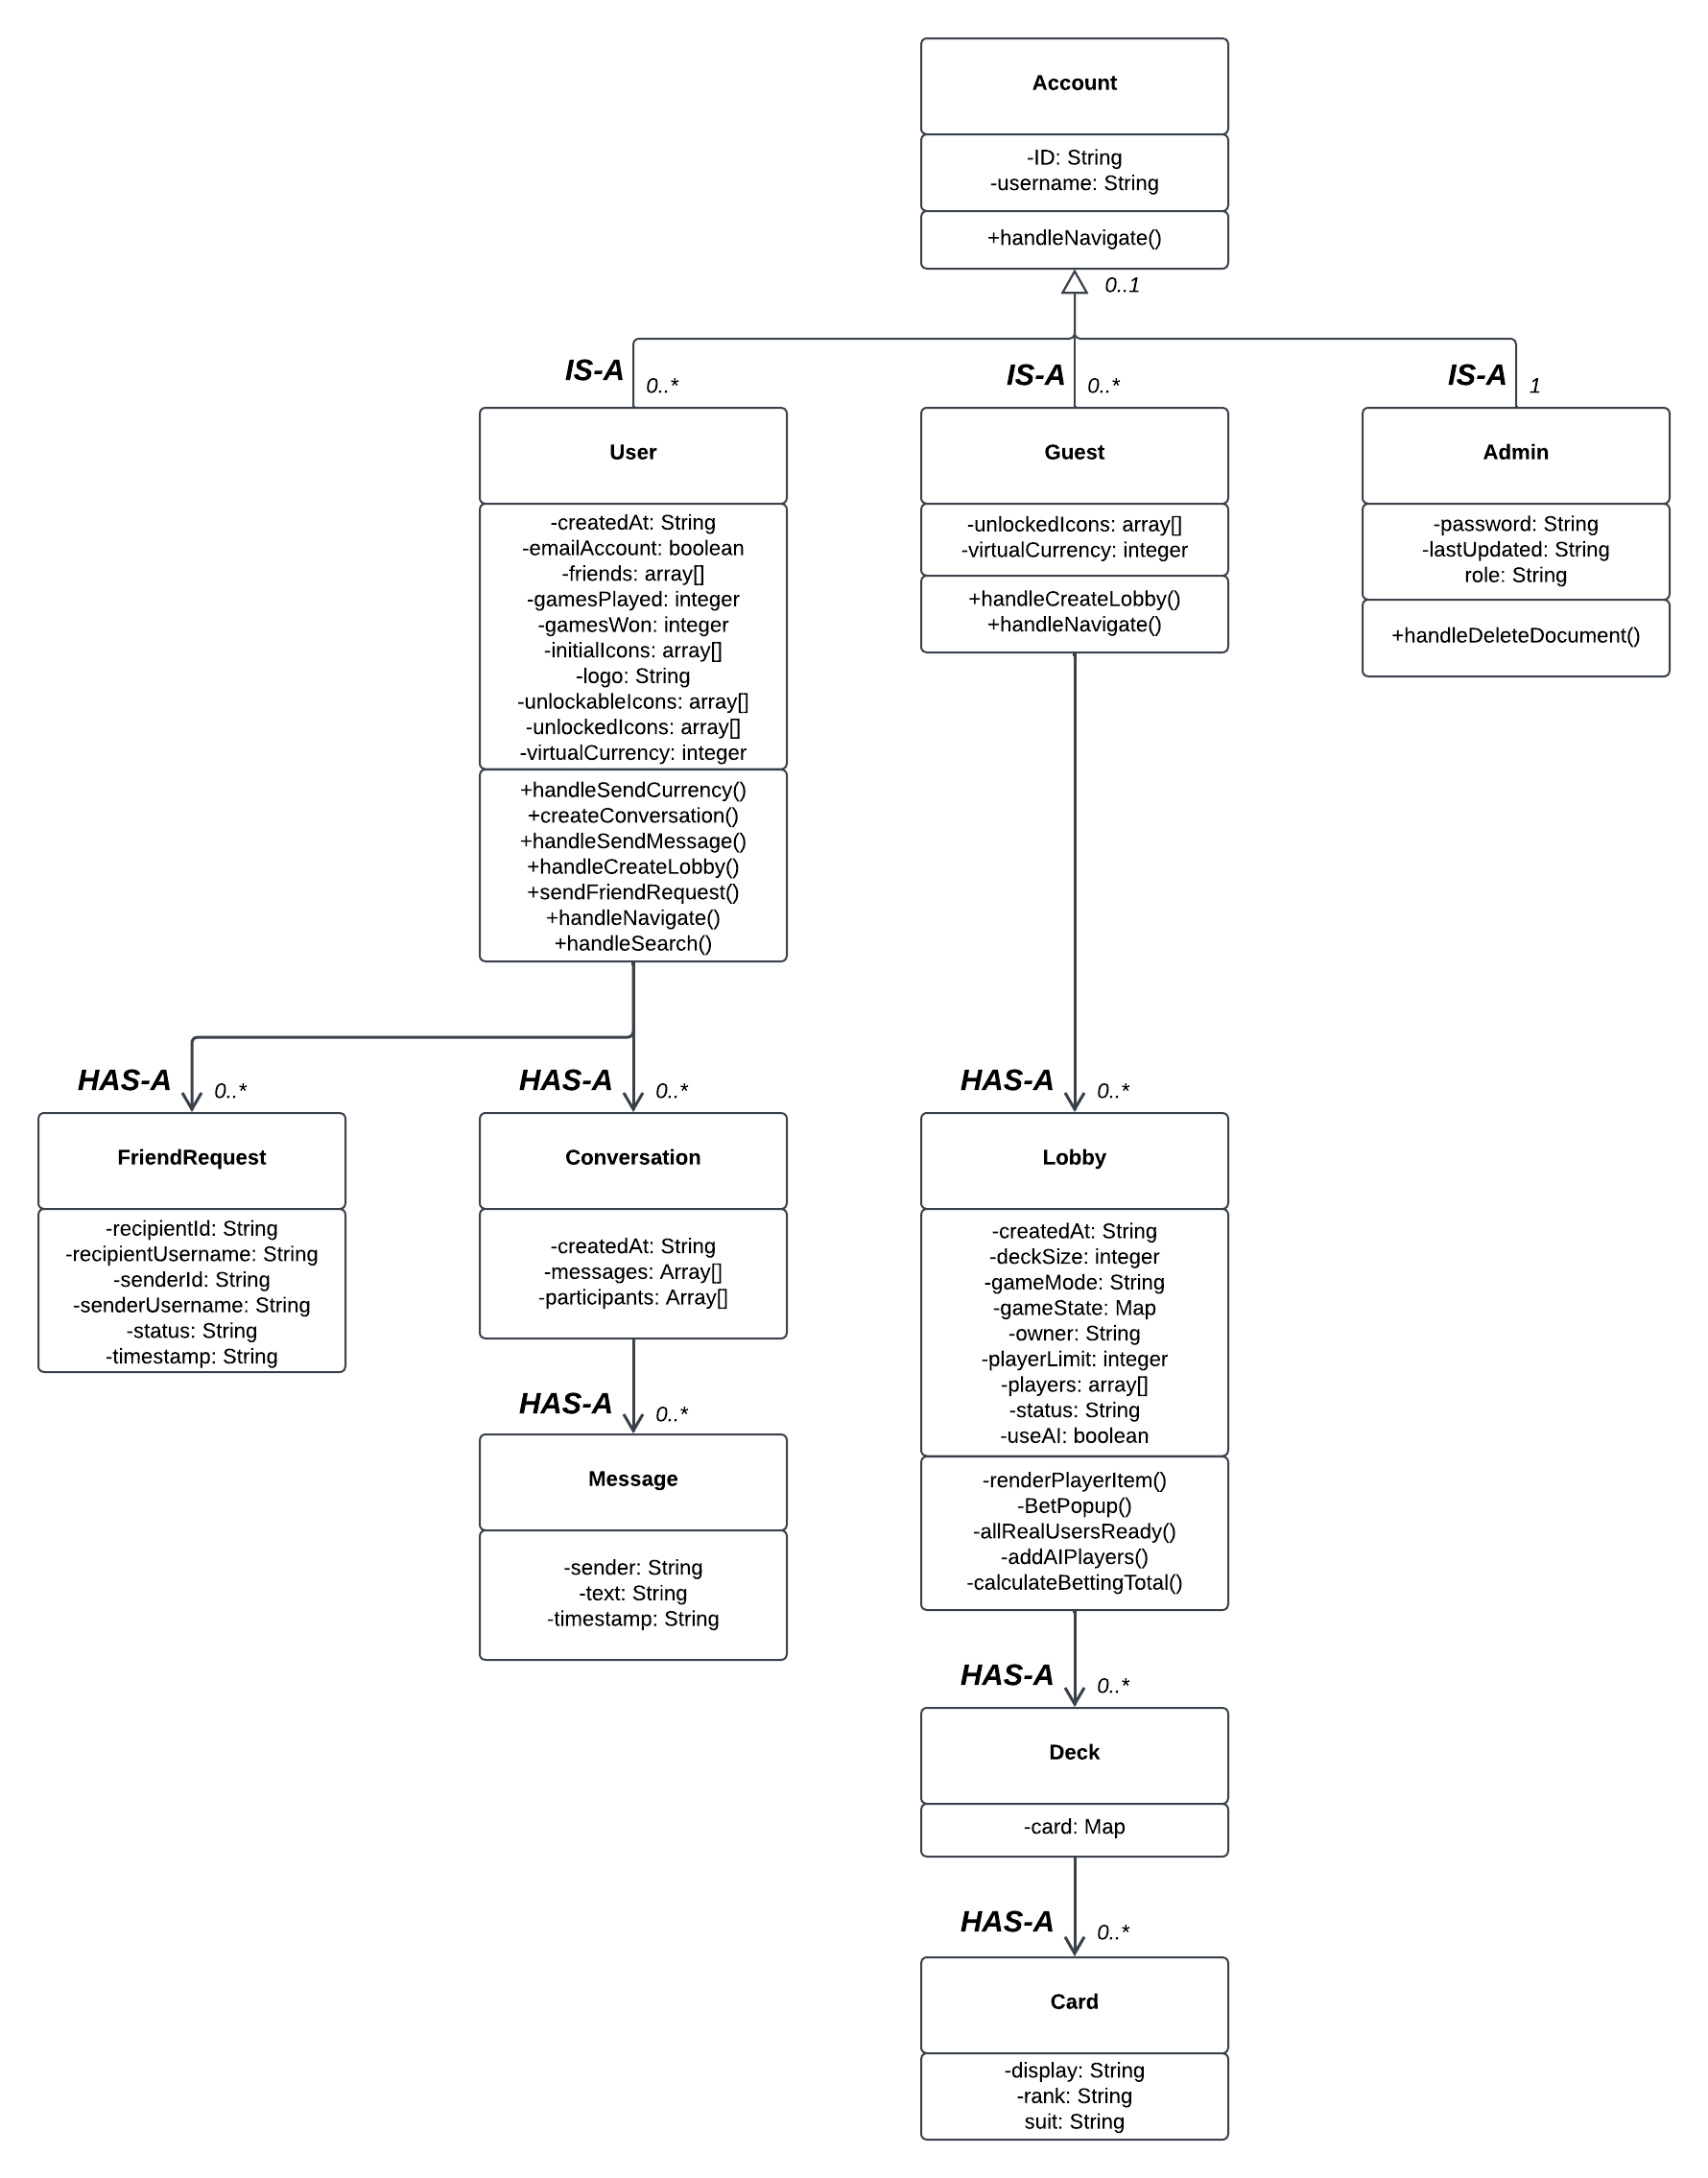
\includegraphics[width=1\linewidth]{CS482 Sequence Diagram Sprint 3.png}
    \caption{UML class diagram showing the system's structure, including key entities, their attributes, methods, and relationships.}
    \label{fig:umlclass}
\end{figure}

\noindent The UML class diagram outlines the system's architecture, showcasing the main classes, their attributes, methods, and relationships. At the top of the hierarchy is the Account class, which acts as the base class with attributes like ID and username and a method for navigation. Three subclasses inherit from Account: User, Guest, and Admin, each with distinct attributes and methods tailored to their specific roles.

\noindent The User class includes attributes such as friends, gamesPlayed, gamesWon, and virtualCurrency, along with methods for sending currency, creating conversations, and managing lobbies. The Guest class serves as a simplified version of the User, with limited attributes and methods focused on navigation and lobby creation. In contrast, the Admin class extends functionality by adding moderation capabilities, such as document deletion and role management.

\noindent The system’s functionality is built around several key components. The FriendRequest class handles friend requests, storing details such as the sender, recipient, and the status of the request. Messaging is managed by the Conversation class, which tracks participants and a collection of messages, with each message including information like the sender, text, and timestamp. The Lobby class oversees game lobbies, managing attributes such as the game mode, game state, and players, while also providing methods for player management, bet calculation, and AI control. Finally, the Deck and Card classes are responsible for managing the game’s deck and individual cards, with attributes defining their ranks, suits, and display properties.

\noindent The diagram highlights important relationships between components: IS-A relationships represent inheritance, while HAS-A relationships show composition or aggregation. It demonstrates how the components work together to support the system's functionality. The focus is on maintaining modularity and scalability, making it easier to expand or adapt the system in the future.
